\chapter{Scenarios}
\section{PIPE interface scenarios}

    \subsection{Electrical Idle} 
    The base spec requires that devices send an Electrical Idle ordered set before Tx+/Tx- goes to the electrical idle state.
    \begin{itemize}
        \item The general rules for entring electrical idle state :
\begin{itemize}
    \item Strat sending EIOS with asserting TxDataK at the same time.
\item the MAC must always align the electrical idle ordered set on the parallel interface so the first byte of the ordered set is always on the low-order data lines (TxDataK[7:0]).

\item Assert TxElecIdle just after sending the EIOS and make sure that TxDataValid is asserted whenever TxElecIdle toggles.

\end{itemize}
\item 
The following timing diagram shows an example of electrical idle entry for gen1,2:

\begin{figure}[H]
  \centering
  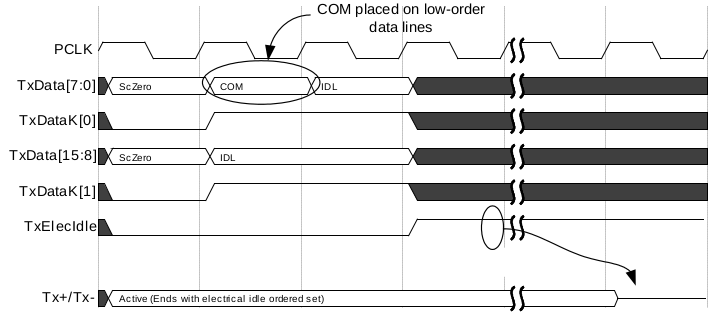
\includegraphics[width=130mm,height=60mm]{images/clk_diagram/EI.png}
  \caption{electrical idle entry for gen1,2}
\end{figure}
\item Some notes on the previous example :
\begin{itemize}
    \item COM appears on the low-order data lines (TxDataK[7:0]).
\item TxElecIdle is asserted after finishing the EIOS.
\item TX+/TX- leaves Active state with the end of EIOS.

\end{itemize}
\item The general rules for leaving electrical idle state :
\begin{itemize}
    \item De-assert TxElecIdle and start sending data.
    \item Make sure TxDataValid is asserted to ensure sampling TxElecIdle.

\end{itemize}
\item The following timing diagram shows an example of electrical idle entry for gen 3:
\begin{figure}[H]
  \centering
  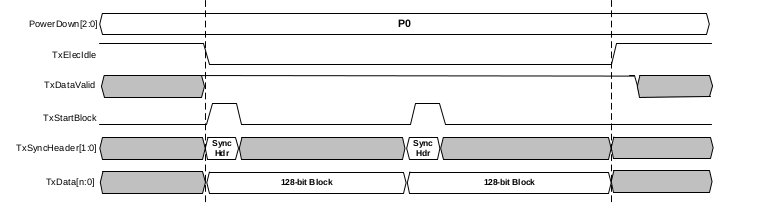
\includegraphics[width=130mm,height=60mm]{images/clk_diagram/EIGen3.png}
  \caption{electrical idle entry for gen3}
  \label{lane}
\end{figure}
Some notes on the previous example:
\begin{itemize}
    \item TxDataValid can assert earlier before TxElecIdle toggles.

    \item TxDataValid can de-assert anytime after TxElecIdle asserts as long as it does not overlap with the next Electrical Idle exit sequence.

    \item TxElecIdle must de-assert at the same clock TxStartBlock asserts.



\end{itemize}
    \end{itemize}
\subsection{Link Equalization Evaluation} 
\begin{itemize}
    \item While in the P0 power state, the PHY can be instructed to perform evaluation of the current TX equalization settings of the link partner.
    \item Basic operation of the equalization evaluation is that:
\begin{itemize}
    \item the MAC requests the PHY to evaluate the current equalization settings by asserting RxEqEval.
    \item When the PHY has completed evaluating the current equalization settings, it asserts PhyStatus for one clock

    \item The PHY drives the LinkEvaluationFeedback signals to the appropriate feedback response.

    \item The MAC must deassert RxEqEval before initiating another evaluation.

    \item To abort an evaluation the MAC de-asserts RxEqEval before the PHY has signaled completion. If the MAC aborts the evaluation the PHY must signal completion as quickly as possible. The MAC ignores returned evaluation values in an abort scenario.
\item If a race condition occurs where the MAC aborts by deasserting RxEqEval on same cycle as the PHY asserts PhyStatus then the PHY shall not take any further action.


\end{itemize}
\item The next figure shows an example of the timings for a successful link equalization evaluation request:
\begin{figure}[H]
  \centering
  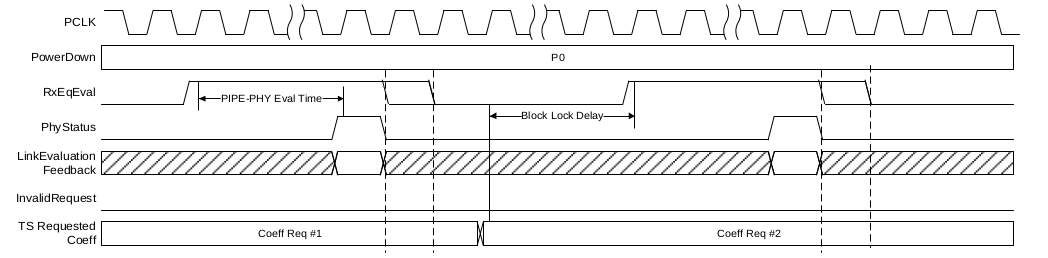
\includegraphics[width=130mm,height=60mm]{images/clk_diagram/eq.png}
  \caption{successful link equalization evaluation request}
  \label{lane}
\end{figure}
\item Notes :
\begin{itemize}
    \item RxEqEval can de-assert at the same clock the corresponding PhyStatus de-asserts or later as long as RxEqEval de-asserts prior to the next RX Equalization Request.

    \item Back-to-back RxEqEval request can happen as close as one clock apart (i.e. RxEqEval can de-assert for one clock before it re-asserts again to start the next RX Equalization request.

    \item Once the MAC has requested link equalization evaluation (by asserting RxEqEval), the MAC must leave RxEqEval asserted until after the PHY has signaled completion by the assertion of PhyStatus unless the MAC needs to abort the evaluation due to high level timeouts or error conditions.

\end{itemize}

    \item The next figure shows PCI Express 3.0 Equalization Evaluation Request Resulting in Invalid Feedback
\begin{figure}[H]
  \centering
  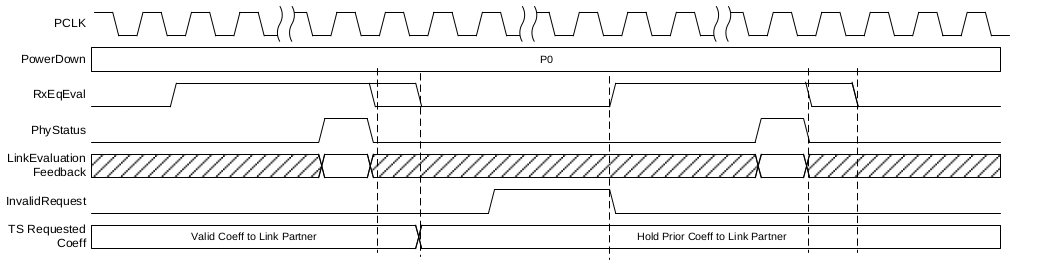
\includegraphics[width=130mm,height=60mm]{images/clk_diagram/eq_v.png}
  \caption{Equalization Evaluation RequestResulting in Invalid Feedback}
  \label{lane}
\end{figure}

\end{itemize}
\subsection{Active PM L0 to L0s and back to L0}  
\begin{itemize}
    \item When the MAC and higher levels have determined that the link should transition to L0s, the MAC transmits an electrical idle ordered set and then has the PHY transmitter go idle and enter P0s.
\item The general rules for entering L0s state from L0:
\begin{itemize}
    \item MAC sends EIOS with the same rules mentioned in the  Electrical Idle section.
\item Just after sending the EIOS, the MAC changes PowerDown[1:0] to 01b indicating transitioning to L0s.
\end{itemize}
The next figure shows the L0s entry for PCIe gen1/2:
\begin{figure}[H]
  \centering
  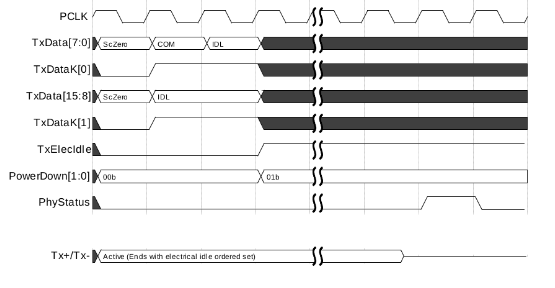
\includegraphics[width=130mm,height=60mm]{images/clk_diagram/l0.png}
  \caption{L0s entry for PCIe gen1/2}
  \label{lane}
\end{figure}
\item The general rules for exiting L0s state to L0:
\begin{itemize}
    \item The MAC transitions the PHY from the P0s state to the P0 state by changing PowerDown[1:0] to 00b.
\item The MAC waits for the PHY to indicate that it is ready to transmit (by the assertion of PhyStatus).
\item Then the MAC begins transmitting Fast Training Sequences (FTS).

\item The next figure shows an example of L0s to L0 transition when the PHY is running at 2.5GT/s.

\begin{figure}[H]
  \centering
  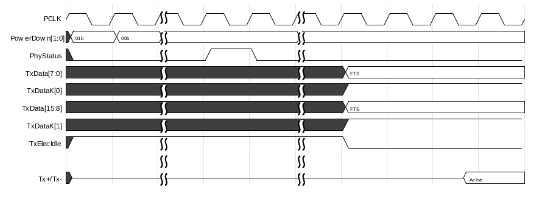
\includegraphics[width=130mm,height=60mm]{images/clk_diagram/l0g.png}
  \caption{ L0s to L0 transition}
  \label{lane}
\end{figure}

\end{itemize}
\end{itemize}
\subsection{reestablish block alignment in recovery state} 
\begin{itemize}
    \item L0 state --> Recovery state due to loss of alignment is detected

    \item In Recovery.RcrLck/cfg, Mac layer assert commandBlockAlignControl bit using messagebus:
\begin{itemize}
    \item Send write committed message to change PHY RX Control4 register to h01 on M2P\_Messagebus.
    \item The phy send ack back for this message on P2M\_Messagebus

    
\end{itemize}
    \item PHY while (commandBlockAlignControl asserted) search for EIEOS to achieve
   block alignment

    \item After Blockalignment is finished

    \item Mac layer go to status L0 and deassert commandBlockAlignControl bit using messagebus:
\begin{itemize}
    \item Send write committed message to change PHY RX Control4 register to h00 on M2P\_Messagebus
\item The phy send ack back for this message on P2M\_Messagebus

\begin{figure}[H]
  \centering
  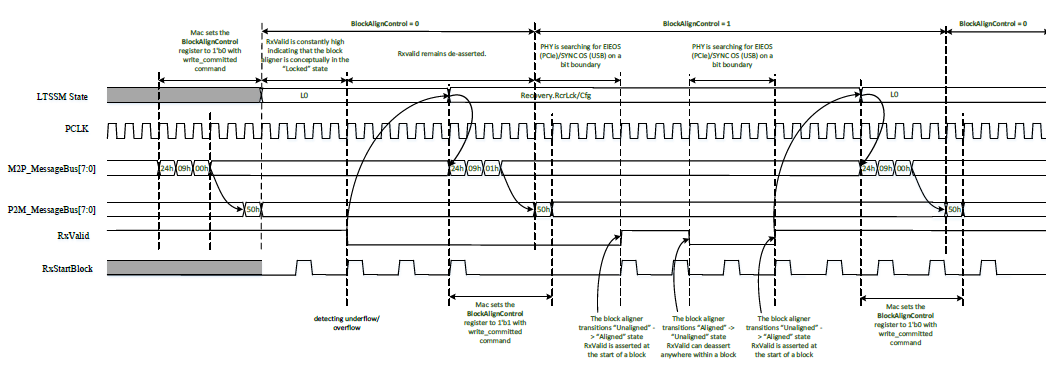
\includegraphics[width=130mm,height=60mm]{images/clk_diagram/recovery.png}
  \caption{reestablish block alignment in recovery state}
  \label{lane}
\end{figure}
\end{itemize}
\end{itemize}
\subsection{RXeqTraining} 
\begin{itemize}
    \item IN Recovery.Equalization Substate,Mac start EqTraining by asserting RXEqTraining bit using messagebus:
\begin{itemize}
    \item Send write committed message to change PHY RX Control1 register[0] to 1 on M2P\_Messagebus
\item The phy send ack back for this message on P2M\_Messagebus 

\end{itemize}
    \item When PHY complete Equalization Training 
    \item PHY layer indicate the status of completion to MAC layer via RxEqualizationDone bit using messagebus:
    \begin{itemize}
        \item  Send write committed message to change RX status register to 1  on P2M\_Messagebus
    \item The Mac send ack back for this message on M2P\_Messagebus


    \end{itemize}
    \begin{figure}[H]
  \centering
  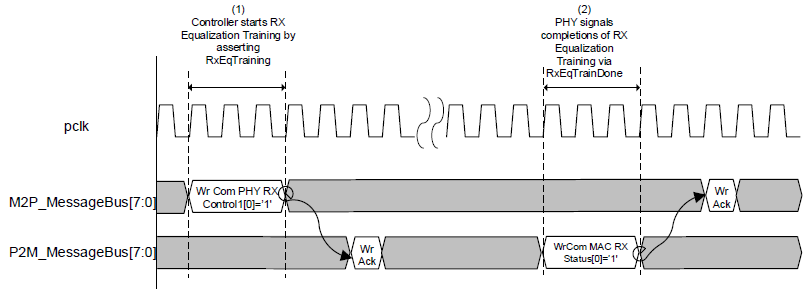
\includegraphics[width=130mm,height=60mm]{images/clk_diagram/RXeqTraining.png}
  \caption{RXeqTraining}
  \label{lane}
\end{figure}
    
\end{itemize}
 \subsection{Reset}
\begin{itemize}
    \item The MAC reset the PHY by asserting Reset signal (active low). 
    \item While Reset is asserted the MAC should have TxDetectRx/Loopback deasserted, TxElecIdle asserted, TxCompliance deasserted and the PowerDown = P1.
    \item For initial power on the MAC must holds PHY in reset until the power and CLK to the PHY are stable.
    \item The PhyStatus is signal is high during reset until reset is deasserted and PCLK is running in operational frequency for one cock and the PHY is in specified power state then it will be deasserted.
    \item When PhyStatus deasserted after the deassertion of the Reset, The MAC can perform any operational sequences.

\begin{figure}[H]
  \centering
  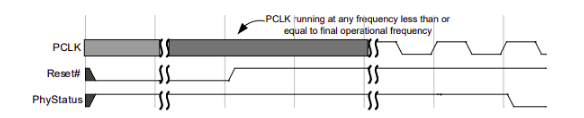
\includegraphics[width=160mm,height=40mm]{images/clk_diagram/reset.png}
  \caption{Reset}
  \label{lane}
\end{figure}
\end{itemize}
\subsection{Updating TxDeemph}  
The TXDeemph is 18-bit variable divided into three parts on (PHY TX Control2, PHY TX Control3, PHY TX Control4) registers.
\begin{itemize}
    \item The MAC sends on M2P\_MessageBus write\_committed to TxControl5 register to make GetLocalPresetCoefficients request for one or more values of LocalPresetIndex to update the TxDeemph value.
This field is used to make dynamic preset coefficient updates.
\item The PHY acknowledge the request by sending write\_ack on the P2M\_MessageBus.
\item The PHY sends three messages on the P2M\_MessageBus to update the LocalPresetCoefficients fields in the (Tx Status0, Tx Status1, Tx Status2) registers.
\item The MAC sends write\_ack message on M2P\_MessageBus to ensure that the LocalPresetCoefficients fields are updated successfully.
\item The MAC sends three messages on the M2P\_MessageBus to the PHY.
\begin{itemize}
    \item Two of them are write\_ucommitted.

    \item One write\_committed to ensure that data are written in the (PHY TX Control2, PHY TX Control3, PHY TX Control4) registers. 

    \item for TxDeemph, the new TxDeemph value must be reflected on the pins within 128ns.
\end{itemize}
\item After the write\_committed for TxDeemph, the new TxDeemph value must be reflected on the pins within 128ns. \newline \newline 

Note: For every GetLocalPresetCoefficients request, there is a 128ns maximum response time for the PHY to return the LocalTxPresetCoefficients value. 

\begin{figure}[H]
  \centering
  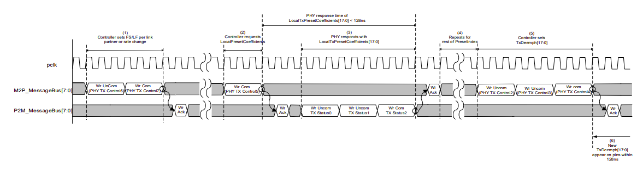
\includegraphics[width=150mm,height=50mm]{images/clk_diagram/deemph.png}
  \caption{Updating TxDeemph}
  \label{lane}
\end{figure}


\end{itemize}
\subsection{Selecting De-emphasis} 
\begin{itemize}
    \item While in the P0 power state and transmitting at 5.0GT/s, 8.0 GT/s, 16 GT/s or 32 GT/s, the PHY can be instructed to change the value of the transmitter equalization.
\item Steps of operation:
\begin{itemize}
    \item The MAC changes the TXDeemph value with the new Tx-De-emphasis value.

    \item If the signaling rate is 5GT/S, the PHY must be capable of transmitting with the new setting within 128 ns.
    \item If the signaling rate is 8.0 GT/s, 16 GT/s, or 32 GT/s, the PHY must be capable of transmitting with the new setting within 256 ns.

\end{itemize}
\begin{figure}[H]
  \centering
  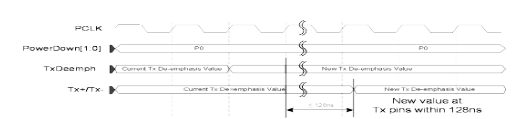
\includegraphics[width=130mm,height=50mm]{images/clk_diagram/de.png}
  \caption{Selecting Tx De-emphasis value}
  \label{lane}
\end{figure}
\end{itemize}
 Polarity Inversion
\begin{itemize}
    \item RxPolarity signal must be asserted to make polarity inversion.

    \item The PHY must invert received data after RxPolarity is asserted.

    \item Inverted data must be showing up on RxData within 20 PCLKs after the assertion of RxPolarity.

    \item Note: The D21.5 symbol when inverted it will be D10.2 symbol as shown in figure.
\begin{figure}[H]
  \centering
  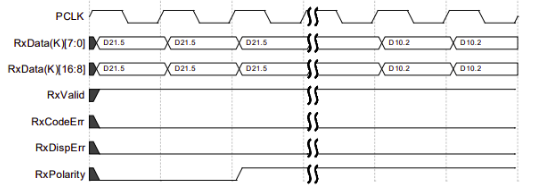
\includegraphics[width=140mm,height=50mm]{images/clk_diagram/p.png}
  \caption{Polarity inversion}
  \label{lane}
\end{figure}
\end{itemize}
\subsection{Signal rate}
\begin{itemize}
    \item Signal rate can be change when PHY in L0 or L1 power state and Tx Electrical IDL is asserted.

    \item After the MAC changes PCLK rate, the change to the PCLK can happen only after the PclkChangeOk has been driven high by the PHY.

    \item The MAC changes the input PCLK and then handshakes by asserting PclkChangeAck.

    \item The PHY responds by the asserting PhyStatus for one input PCLK cycle and deasserts PclkChangeOk on the trailing edge of PhyStatus.

    \item The MAC deasserts PclkChangeAck when PclkChangeOk is sampled low and may deassert Tx Electrical IDL.

\begin{figure}[H]
  \centering
  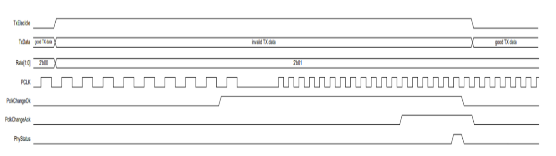
\includegraphics[width=130mm,height=50mm]{images/clk_diagram/rate.png}
  \caption{signal rate}
  \label{lane}
\end{figure}
\end{itemize}
\subsection{Error Detection} 
\begin{itemize}
    \item The PHY is responsible for detecting receive errors of several types, these errors are signalled to the MAC layer using the receiver status signals (RxStatus[2:0]).

    \item When a receive error occurs, the appropriate error code is asserted for one clock cycle at the point in the data stream across the parallel interface closest to where the error actually occurred.

    \item There are four error conditions that can be encoded on the RxStatus signals.

    \item If more than one error should happen to occur on a receive byte, the errors should be signaled with the priority shown below.
\begin{itemize}
    \item 8B/10B decode error or block code error (RxStatus=100b).

    \item Elastic Buffer overflow (RxStatus=101b).

    \item Elastic Buffer underflow (RxStatus=110b).

    \item Disparity errors (RxStatus=111b).

\end{itemize}
\end{itemize}
\subsection{8B/10B Decode Errors} 
\begin{itemize}
    \item For a detected 8B/10B decode error, the PHY should place an EDB symbol in the data stream in place of the bad byte, and encode RxStatus with a decode error during the clock cycle when the effected byte is transferred across the parallel interface. 

    \item For greater than 8-bit interface, if the bad on the lower byte lane, one of the other bytes may have bad disparity, but the 8B/10B error has the precedence.

    \item In the example below, the receiver is receiving a stream of bytes Rx-a through Rx-z, and byte Rx-f has an 8B/10B decode error, in the place of that byte, the PHY places an EDB on the parallel interface and sets RxStatus to the 8B/10B decode error code.
\begin{figure}[H]
  \centering
  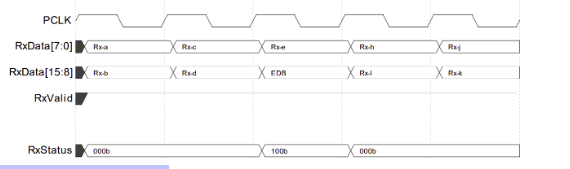
\includegraphics[width=130mm,height=50mm]{images/clk_diagram/dr.png}
  \caption{8B/10B Decode Errors}
  \label{lane}
\end{figure}
\end{itemize}
\subsection{Disparity Errors} 
\begin{itemize}
    \item For a detected disparity error the PHY should assert RxStatus with the disparity error code during the clock cycle when the affected byte is transferred across the parallel interface.
 
    \item For greater than 8-bit interfaces, it is not possible to discern which byte (or possibly both) had the disparity error.

    \item In the example below, the receiver detected a disparity error on either (or both) Rx-e or Rx-f data bytes and indicates this with the assertion of RxStatus.

\begin{figure}[H]
  \centering
  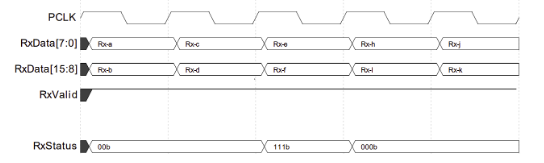
\includegraphics[width=130mm,height=50mm]{images/clk_diagram/disparity.png}
  \caption{Disparity Errors}
  \label{lane}
\end{figure}
\item  Note: MACs often treat 8B/10B errors and disparity errors identically.
\end{itemize}


\subsection{Elastic Buffer Errors}
\subsubsection{Elastic Buffer Underflow}

\begin{itemize}
    \item For elastic buffer errors, an underflow should be signaled during the clock cycle or clock cycles when a spurious symbol is moved across the parallel interface, the symbol moved across the interface should be the EDB symbol.

    \item In the timing diagram below, the PHY is receiving a repeating set of symbols Rx-a thru Rx-z, the elastic buffer underflows causing the EDB symbol to be inserted between Rx-g and Rx-h symbols, the PHY drives RxStatus to indicate buffer underflow during the clock cycle when the EDB is presented on the parallel interface.

\end{itemize}




\begin{figure}[H]
  \centering
  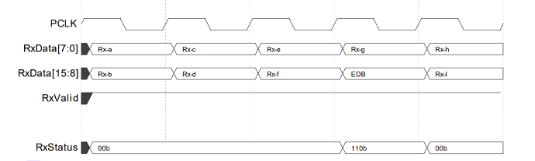
\includegraphics[width=130mm,height=50mm]{images/clk_diagram/underflow.png}
  \caption{Elastic Buffer Underflow}
  \label{lane}
\end{figure}
\subsubsection{Elastic Buffer Overflow}
\begin{itemize}
    \item For an elastic buffer overflow, the overflow should be signaled during the clock cycle where the dropped symbol or symbols would have appered in the data stream.

    \item For the 16-bit interface it is not possible, or necessary, for the MAC to determine exactly where in the data stream the symbol was dropped.

    \item In the timing diagram below, the PHY is receiving a repeating set of symbols Rx-a thru Rx-z, the elastic buffer overflows causing the symbol Rx-g to be discarded, The PHY drives RxStatus to indicate buffer overflow during clock cycle when Rx-g would have appeared on the parallel interface.     

\end{itemize}




\begin{figure}[H]
  \centering
  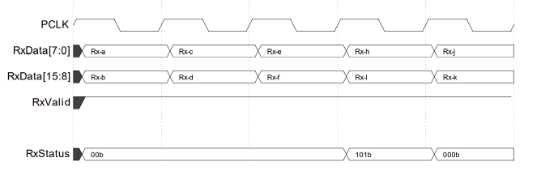
\includegraphics[width=130mm,height=50mm]{images/clk_diagram/overflow.png}
  \caption{Elastic Buffer Overflow}
  \label{lane}
\end{figure}
\subsection{Receiver detection}
\begin{itemize}
    \item While in the P1 power state the PHY can be instructed to perform a  receiver detection operation to determine if there is a receiver at the other end of the link.

    \item Basic operation of receiver detection is that MAC requests the PHY to do receiver detect sequence by asserting TxDetectRx/Loopback.

    \item When the PHY has completed the receiver detect sequence, it asserts PhyStatus for one clock and drives the RxStatus signals to the appropriate code.

    \item After the receiver detection has completed, the MAC must deassert TxDetectRx/Loopback before initiating another receiver detection.

    \item Once the MAC has requested a receiver detect sequence the MAC must leave TxDetectRx/Loopback asserted until after the PHY has signaled completion by the assertion of Phystatus.
\end{itemize}




\begin{figure}[H]
  \centering
  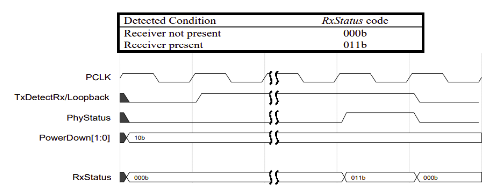
\includegraphics[width=130mm,height=50mm]{images/clk_diagram/detection.png}
  \caption{Receiver detection}
  \label{lane}
\end{figure}

\subsection{128b/130b Encoding and Block synchronization}
\begin{itemize}
    \item For every block (usually 128 bits) that is moved across the PIPE TxData interface at the 8.0 GT/s rate, 16 GT/s rate, or 32 GT/s rate, TxSyncHeader signal is asserted to Provide the Sync Header for the PHY to use in the next 128b block.

    \item The MAC must assert the TxDataValid signal to indicate that PHY will use the data.
    \item TxStartBlock signal is asserted to allow the MAC to tell PHY the starting byte for a 128b block.

    \item TxElecIdle signal Forces Tx output to electrical idle when asserted.

    \item For every block (usually 128 bits) that is moved across the PIPE RxData interface at the 8.0 GT/s rate, 16 GT/s rate, or 32 GT/s rate, RxSyncHeader signal is asserted to Provide the Sync Header for the MAC to use in the next 128b block.

    \item The PHY must assert the RxDataValid signal to indicate that MAC will use the data.

    \item RxStartBlock signal is asserted to Allows the PHY to tell MAC the starting byte for a 128b block.

    \item RxElecIdle signal Indicates receiver detection of an electrical idle when asserted.
\end{itemize}
\begin{figure}[H]
  \centering
  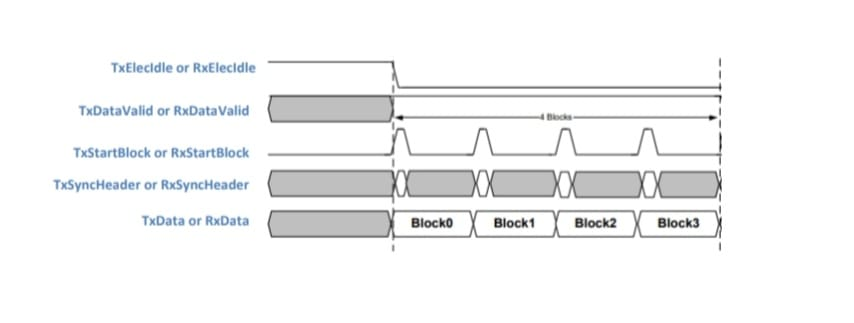
\includegraphics[width=130mm,height=50mm]{images/clk_diagram/end.jpeg}
  \caption{128b/130b Encoding and Block synchronization}
  \label{lane}
\end{figure}

% \begin{figure}[H]
%   \centering
%   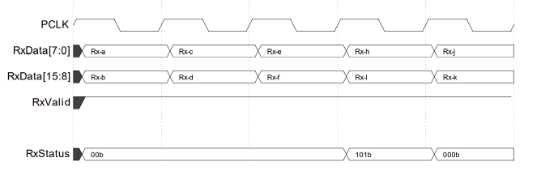
\includegraphics[width=130mm,height=50mm]{images/clk_diagram/overflow.png}
%   \caption{Elastic Buffer Overflow}
%   \label{lane}
% \end{figure}